%!TEX root = ../dokumentation.tex

\chapter{Server}
\label{ch:Server}

Der Befehl "npm run dev", der auch in der package.json beschrieben ist und der innerhalb der Dockerfile aufgerufen wird, startet den Node-Server. Dafür wird per nodemon die Datei server.js angesprochen und diese startet dann den Server auf Port 3000.

\begin{figure}[h]
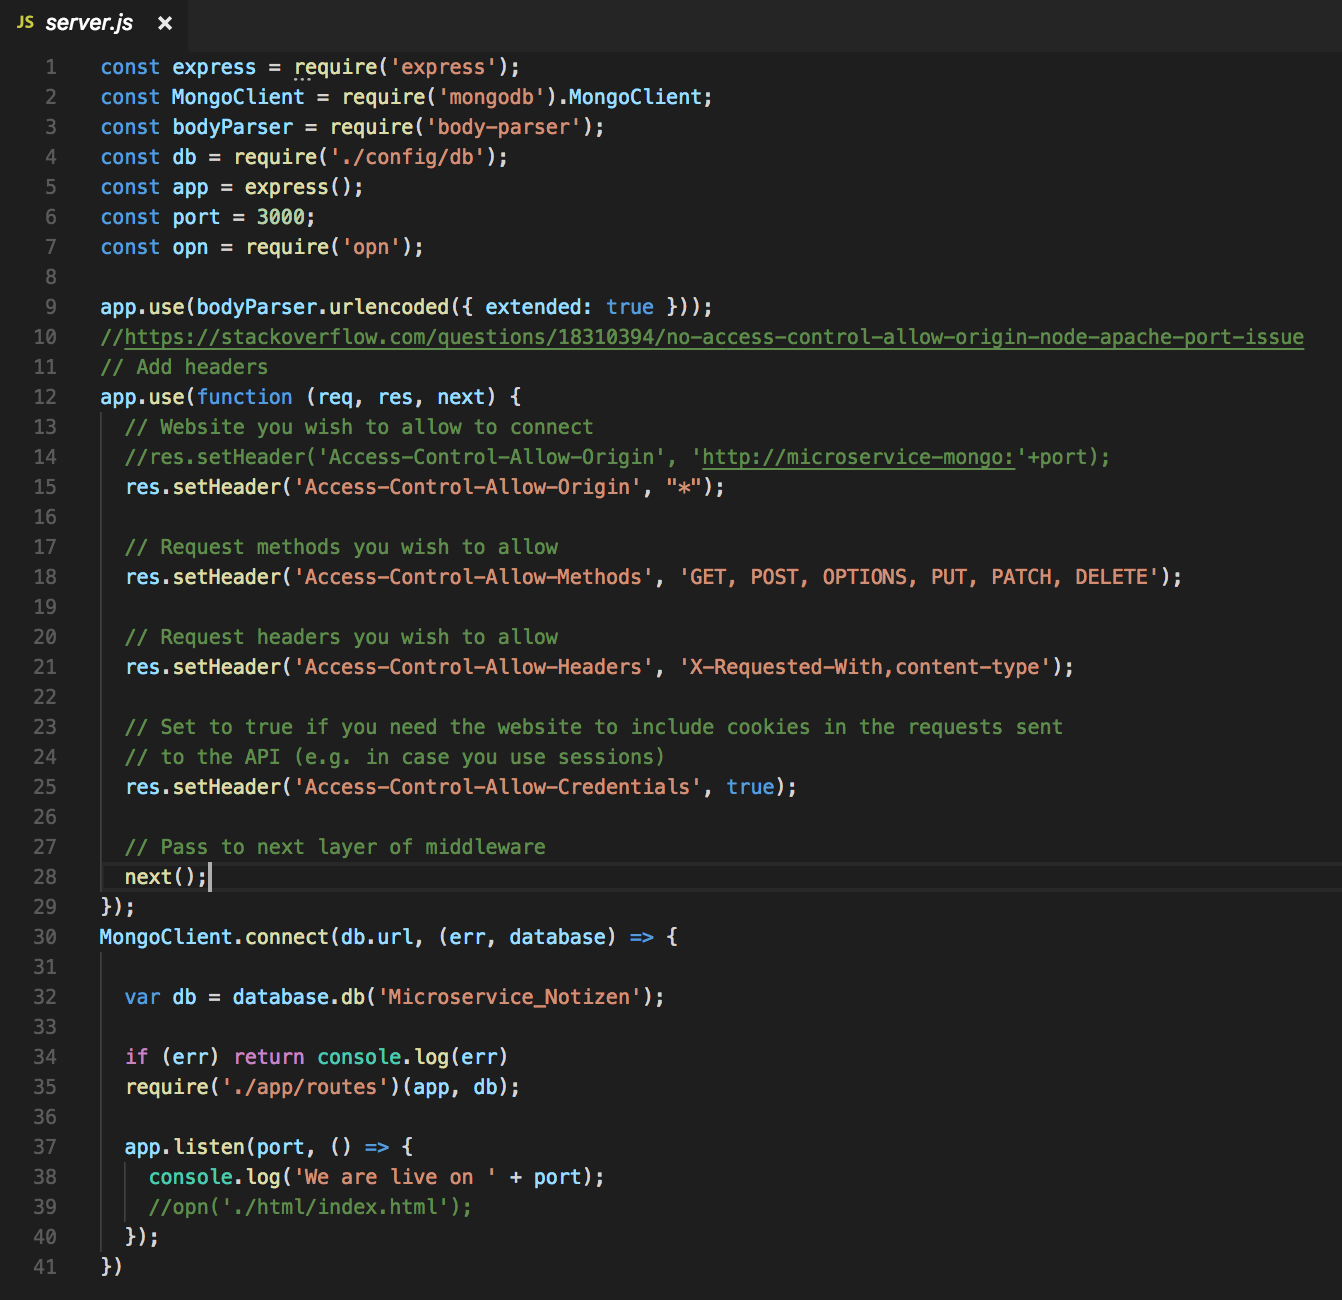
\includegraphics[height=0.9\textwidth]{ServerMain.png}
\vspace{3pt}
\caption{Schaubild\footnotemark}
\label{fig:blueant}
\end{figure}


In den Imports innerhalb der oberen Zeilen 1 bis 7 werden die benötigten Module geladen und dem Server zur Verfügung gestellt.

Die darauffolgenden Zeilen 9 bis 29 werden vom BodyParser benötigt und liefern die benötigten Daten zur Verarbeitung von Requestbodies.

Ab Zeile 30 wird der Node-Server definiert. Dafür wird die Datenbankverbindung definiert, der Import der Routes vollzogen und dem Server mitgeteilt auf welche Ports er hören soll und wie er das Empfangene an Hand der Routes verarbeiten soll.